\documentclass[../poma-notes.tex]{subfiles}

\begin{document}

本章基于黎曼积分的定义,该定义明确的取决于实线的层次结构。因此首先我们将探讨区间内实值函数的积分,然后再是复数与向量函数的积分,
而非区间积分将会在第十与十一章进行探讨。

\subsection*{Definition and Existence of the Integral}

\begin{definition}
  Let $[a,b]$ be a given interval. By a \textit{partition} $P$ of $[a,b]$ we mean a finite set of points
  $x_0, x_1, \dots, x_n$, where
  \[
    a = x_0 \le x_1 \le \cdots \le x_{n-1} \le x_n = b.
  \]

  We write
  \[
    \delta x_i = x_i - x_{i-1} \qquad (i=1,\dots,n).
  \]
  Now suppose $f$ is a bounded real function defined on $[a,b]$. Corresponding to each partition $P$ of
  $[a,b]$ we put
  \begin{align*}
    \begin{split}
      M_i &= \sup f(x) \qquad (x_{i-1} \le x \le x_i), \\
      m_i &= \inf f(x) \qquad (x_{i-1} \le x \le x_i), \\
      U(P,f) &= \sum_{i=1}^{n} M_i \delta x_i, \\
      L(P,f) &= \sum_{i=1}^{n} m_i \delta x_i,
    \end{split}
  \end{align*}
  and finally
  \begin{equation}
    \tint_{a}^{b} f \,dx = \inf\, U(P, f),
  \end{equation}
  \begin{equation}
    \bint_{a}^{b} f \,dx = \sup\, L(P, f),
  \end{equation}
  where the inf and the sup are taken over all partitions $P$ of $[a,b]$. The left members of (1) and (2)
  are called the \textit{upper} and \textit{lower Riemann integrals} of $f$ over $[a,b]$, respectively.

  If the upper and lower integrals are equal, we say that $f$ is \textit{Riemann-integrable} on $[a,b]$,
  we write $f \in \mathscr{R}$ (that is, $\mathscr{R}$ denotes the set of Riemann-integrable functions),
  and we denote the common value of (1) and (2) by
  \begin{equation}
    \int_{a}^{b}f\,dx,
  \end{equation}
  or by
  \begin{equation}
    \int_{a}^{b}f(x)\,dx.
  \end{equation}

  This is the \textit{Riemann integral} of $f$ over $[a,b]$. Since $f$ is bounded, there exist two numbers,
  $m$ and $M$, such that
  \[
    m \le f(x) \le M \qquad (a \le x \le b).
  \]
  Hence, for every $P$,
  \[
    m(b-a) \le L(P, f) \le U(P, f) \le M(b-a),
  \]
  so that the numbers $L(P, f)$ and $U(P, f)$ form a bounded set. This shows that \textit{the upper and lower
    integrals are defined for every} bounded function $f$. The question of their equality, and hence the question
  of the integrability of $f$, is a more delicate one. Instead of investigating it separately for the Riemann
  integral, we shall immediately consider a more general situation.
\end{definition}

\begin{anote}
  \begin{enumerate}
    \item \textbf{Partition}: $[a, b]$ 区间的\textbf{分割}。
    \item \textbf{Sub-interval}:每个 $[x_i, x_{i+1}]$ 即 partition 的 \textbf{子区间}。
    \item \textbf{Mesh}/\textbf{Norm}:一个分割的\textbf{标准},即最长的那个子区间 $\max(x_{i+1} - x_i),\ i\in[0, n-1]$。
    \item \textbf{Tagged partition}:\textbf{取样分割},$P(x,t)$ 指在进行分割 $a = x_0 < x_1 < x_2 < \dots < x_n = b$ 后,
          与每一个子区间中 $[x_i,x_{i+1}]$ 取出一点 $x_i \le t_i \le x_{i+1}$。
    \item \textbf{Refinement}:\textbf{精细化分割}。假设两个分区 $P(x,t)$ 与 $Q(y,s)$ 皆为区间 $[a,b]$ 的分区。对于每个整数
          $i,\ i\in[0,n]$,存在一个整数 $r(i)$ 满足 $x_i = y_{r(i)}$,以及对于某 $j,\ j\in[r(i),r(i+1)]$ 满足 $t_i = s_j$,
          那么我们可以将 $Q(y,s)$ 称为 $P(x,t)$ 的精细化分割。简言之,$Q(y,s)$ 是在 $P(x,t)$ 的基础上添加一些分点和标记。那么可以在此
          区间的所有采样分割中定义一个 \href{https://en.wikipedia.org/wiki/Partially_ordered_set}{偏序关系 partially ordered set},
          称作\say{精细}。
    \item \textbf{Riemann sum}:\textbf{黎曼和}。令 $f$ 为定义在区间 $[a,b]$ 上的实值函数,$f$ 的黎曼和取决于取样分割 $x_0,\dots,x_n$,
          $t_0,\dots,t_{n-1}$:
          \[
            \sum_{i=0}^{n-1}f(t_i)(x_{i+1}-x_i)
          \]
          其中 $f(t_i)$ 视作高度,$x_{i+1} - x_i$ 视作宽度,而黎曼和则是所有带符号的矩形区域之和。
    \item \textbf{Upper \& lower Riemann Sums}:\textbf{上黎曼和} $U(P,f) = \sum_{i=1}^{n} M_i \delta x_i$
          与\textbf{下黎曼}和 $L(P,f) = \sum_{i=1}^{n} m_i \delta x_i$,详见下图。
    \item \textbf{Upper \& lower Riemann integrals}:\textbf{上黎曼积分}与\textbf{下黎曼积分}。严格定义如下:$S$ 是函数 $f$
          在闭区间 $[a,b]$ 上的黎曼积分,当且仅当对于任意的 $\varepsilon > 0$,都存在 $\delta > 0$,使得对于任意的取样分割
          $x_0,\dots,x_n$,$t_0,\dots,t_{n-1}$,只要它的子区间长度最大值 $\lambda \le \delta$,就有
          \[
            \biggl| \sum_{i=0}^{n-1} f(t_i)(x_{i+1} - x_i) - S \biggr| < \varepsilon
          \]
    \item \textbf{Riemann-integrable}:\textbf{黎曼可积}。对于一个函数 $f$,如果在闭区间 $[a,b]$ 上,无论怎样进行取样分割,
          只要它的子区间长度最大值足够小,函数 $f$ 的黎曼和都会趋向于一个确定的值,那么 $f$ 在闭区间 $[a,b]$ 上的黎曼积分存在,
          并且定义为黎曼和的极限,这时候称函数 $f$ 为黎曼可积的(上下黎曼积分相等时,$f$ 在区间 $[a,b]$ 上黎曼可积)。
          然而这个定义的缺陷是没有可操作性,因为要检验所有 $\lambda \le \delta$ 的取样分割是很难做到的(接下来的定义更具有普适性)。
  \end{enumerate}
\end{anote}

\begin{figure}[htp]
  \centering
  \subfloat[$n=10$]{
    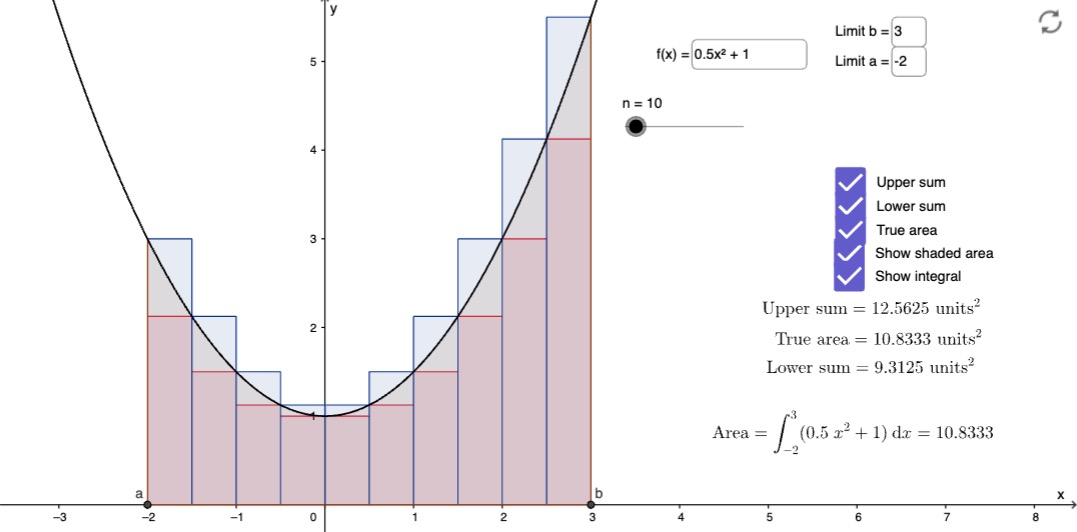
\includegraphics[width=0.4\textwidth]{\subfix{../images/UpperAndLowerRiemannSums1.png}}
  }
  \hfill
  \subfloat[$n=50$]{
    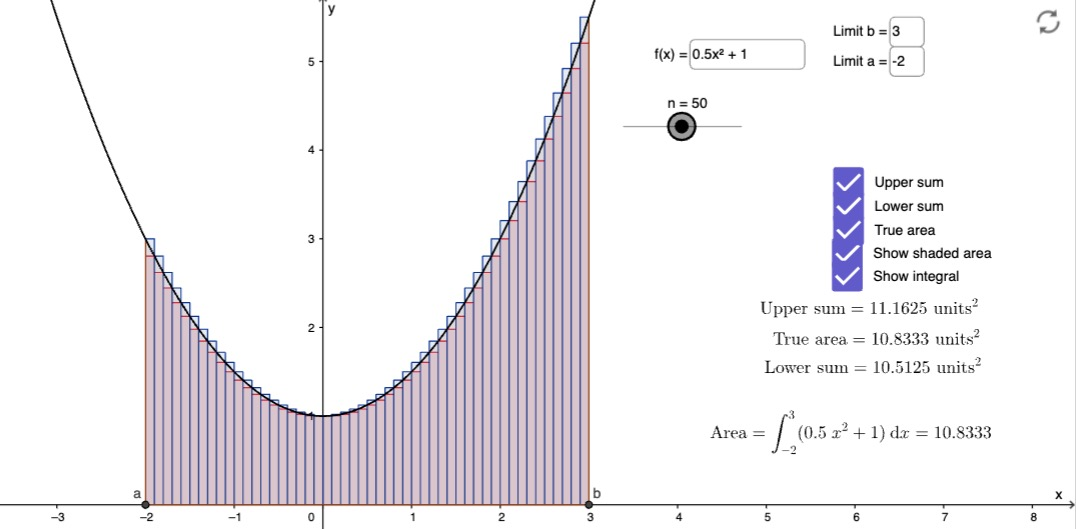
\includegraphics[width=0.4\textwidth]{\subfix{../images/UpperAndLowerRiemannSums2.png}}
  }
  \caption*{Upper and lower Riemann sums}
\end{figure}

\begin{definition}
  Let $\alpha$ be a monotonically increasing function on $[a,b]$ (since $\alpha(a)$ and $\alpha(b)$ are finite,
  it follows that $\alpha$ is bounded on $[a,b]$). Corresponding to each partition $P$ of $[a,b]$, we write
  \[
    \Delta\alpha_i = \alpha(x_i) - \alpha(x_{i-1}).
  \]
  It is clear that $\Delta\alpha_i \ge 0$. For any real function $f$ which is bounded on $[a,b]$ we put
  \begin{align*}
    \begin{split}
      U(P,f,\alpha) &= \sum_{i=1}^{n} M_i \delta\alpha_i, \\
      L(P,f,\alpha) &= \sum_{i=1}^{n} m_i \delta\alpha_i,
    \end{split}
  \end{align*}
  where $M_i, m_i$ have the same meaning as in Definition 6.1, and we define
  \begin{equation}
    \tint_a^b f\,d\alpha = \inf U(P,f,\alpha),
  \end{equation}
  \begin{equation}
    \bint_a^b f\,d\alpha = \sup L(P,f,\alpha),
  \end{equation}
  the inf and sup again being taken over all partitions.

  If the left members of (5) and (6) are equal, we denote their common value by
  \begin{equation}
    \int_a^b f\,d\alpha
  \end{equation}
  or sometimes by
  \begin{equation}
    \int_a^b f(x)\,d\alpha(x).
  \end{equation}

  This is the \textit{Riemann-Stieltjes integral} (or simply the \textit{Stieltjes integral}) of $f$ with respect to
  $\alpha$, over $[a,b]$.

  If (7) exists, i.e., if (5) and (6) are equal, we say that $f$ is integrable with respect to $\alpha$, in the Riemann
  sense, and write $f\in\mathscr{R}(\alpha)$.

  By taking $\alpha(x)=x$, the Riemann integral is seen to be a special case of the Riemann-Stieltjes integral. Let us
  mention explicitly, however, that in the general case $\alpha$ need not even be continuous.

  A few words should be said about the notation. We prefer (7) to (8), since the letter $x$ which appears in (8) adds nothing
  to the content of (7). It is immaterial which letter we use to represent the so-called \say{variable of integration.}
  For instance, (8) is the same as
  \[
    \int_a^b f(y)\,d\alpha(y).
  \]
  The integral depends on $f, \alpha, a$ and $b$, but not on the variable of integration, which may as well be omitted.

  The role played by the variable of integration is quite analogous to that of the index of summation: The two symbols
  \[
    \sum_{i=1}^{n} c_i, \qquad \sum_{k=1}^{n} c_k
  \]
  mean the same thing, since each means $c_1 + c_2 + \cdots + c_n$.

  Of course, no harm is done by inserting the variable of integration, and in many cases it is actually convenient to do so.

  We shall now investigate the existence of the integral (7). Without saying so every time, $f$ will be assumed real and
  bounded, and $\alpha$ monotonically increasing on $[a,b]$; and, when there can be no misunderstanding, we shall write $\int$
  in place of $\int_a^b$.
\end{definition}

\begin{anote}
  取 $\alpha(x) = x$ 时,Riemann 积分被视为 Riemann-Stieltjes 积分的一个特例。不过一般情况下,$\alpha$ 甚至不一定是连续的。
\end{anote}

\newpage

\begin{anote}
  \textbf{几何解释}

  在一个 $x,\ f(x)\ \text{以及}\ g(x)$ 三维的正交坐标系中,如果 $g-x$ 面是水平方向的,且 $f$ 的是正向上的,那么 $(x,f,g)$ 的表面可以视为一个
  弯曲的栅栏(下图紫色部分)。栅栏的的弯曲方向取决于 $g(x)$ 的走向,而其高度则是取决于给定的 $f(x)$。该栅栏是 $g$-sheet 的一部分(例如,$g$ 曲线在
  $f$ 轴方向延伸),其被 $g-x$ 平面与 $f$-sheet 所界限。而 Riemann-Stieltjes 积分则是该栅栏投影到 $f-g$ 平面上的面积 -- 实际上就是其
  \say{影子}($x=0,f,g$ 平面,即最左侧平面)。
\end{anote}

\begin{figure}[h]
  \centering
  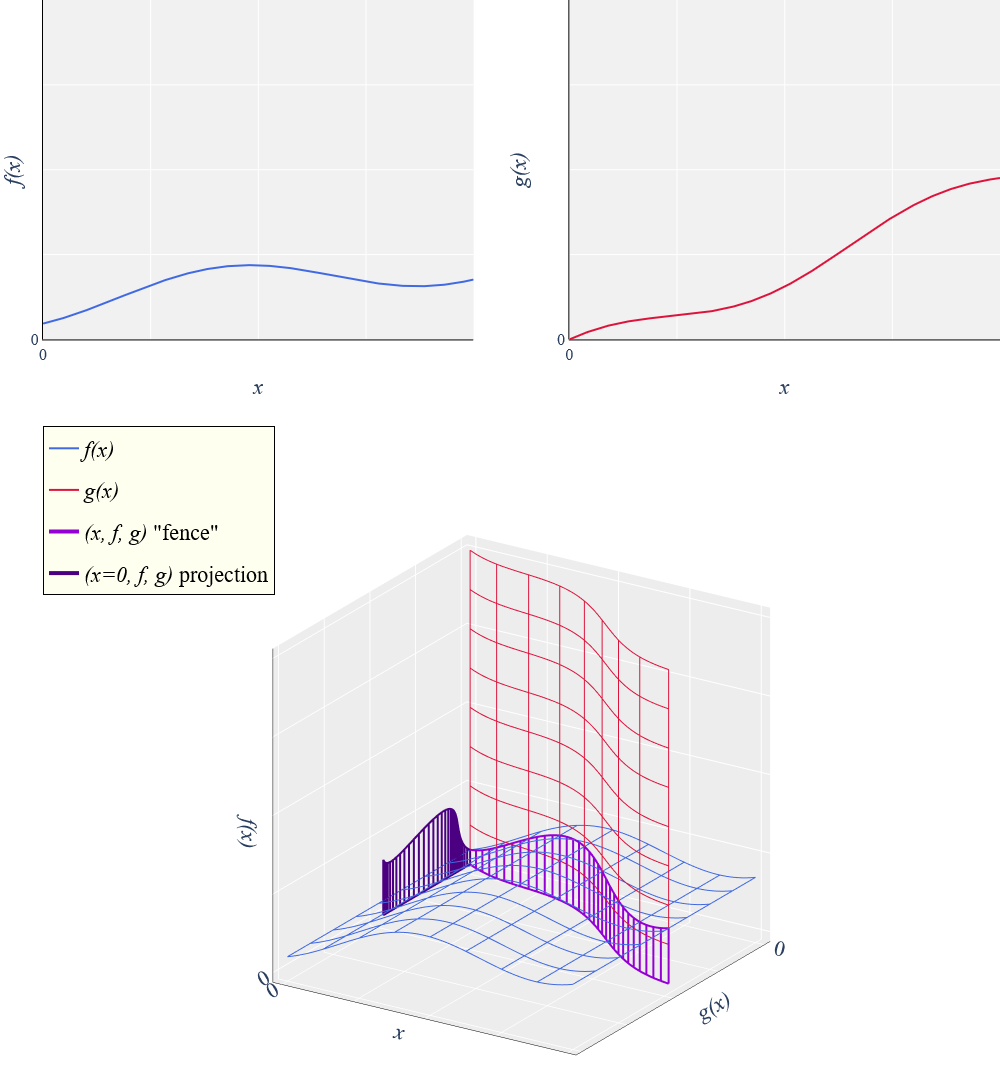
\includegraphics[width=0.9\textwidth]{\subfix{../images/Basic_geometry_of_riemann-stieljes_integral_f_g_x.png}}
\end{figure}

% TODO

% \begin{figure}[h]
%   \centering
%   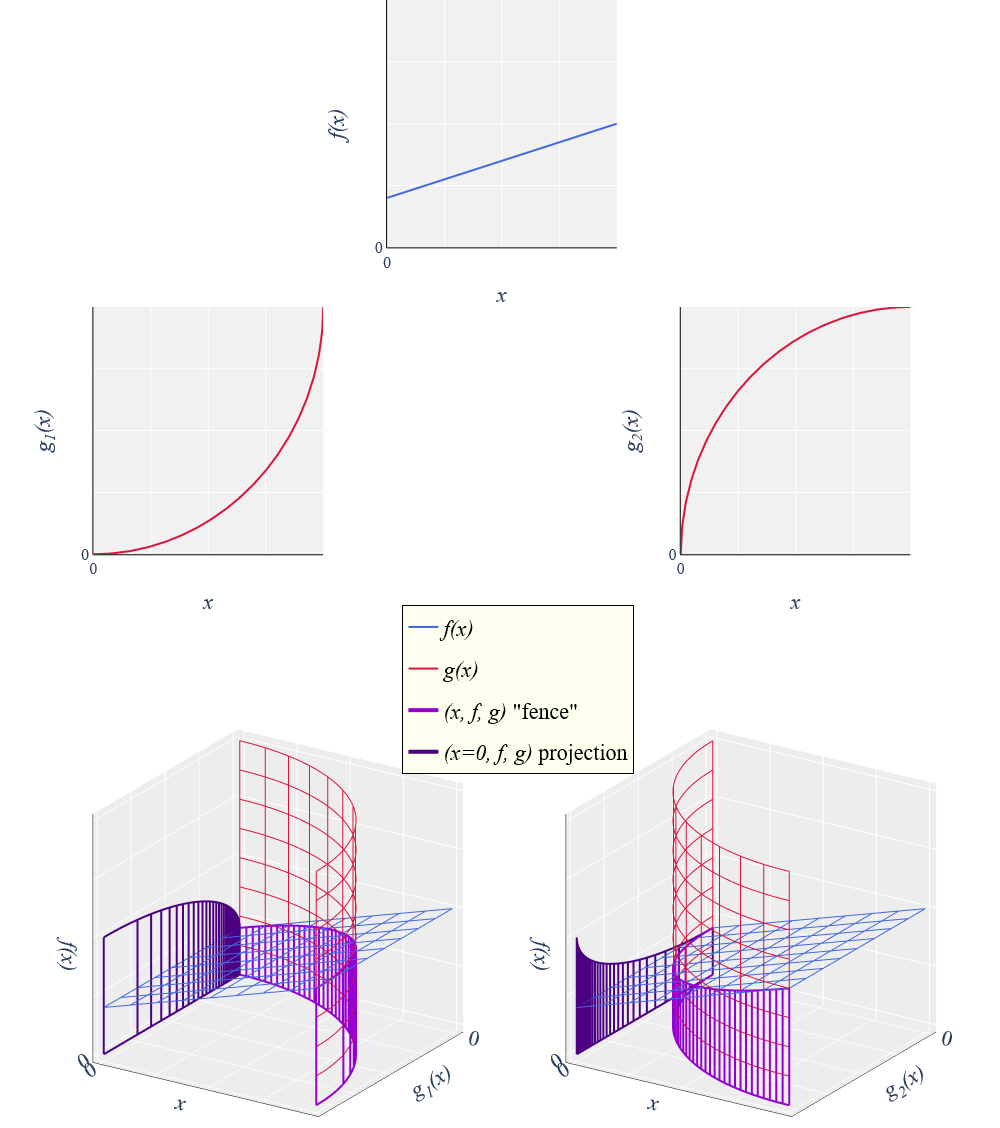
\includegraphics[width=0.4\textwidth]{\subfix{../images/Curvature_effects_on_geometry_of_riemann-stieljes_integral_f_g_x.png}}
% \end{figure}

% \begin{figure}[h]
%   \centering
%   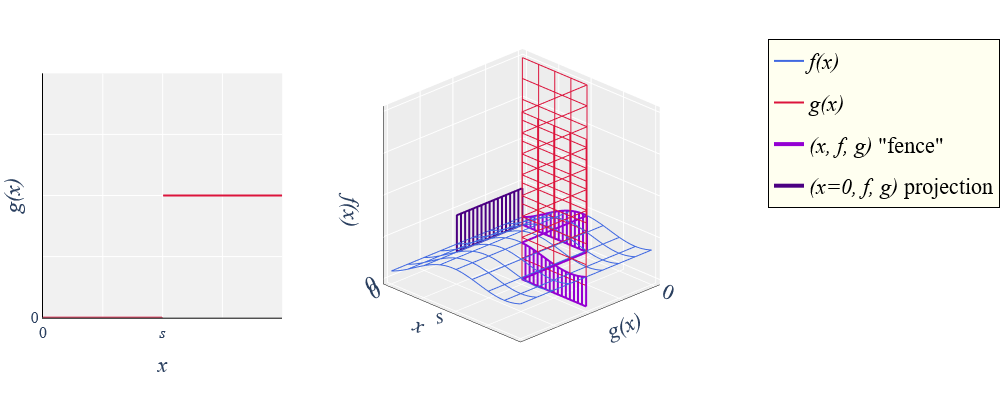
\includegraphics[width=0.4\textwidth]{\subfix{../images/Step_function_effect_on_geometry_of_riemann-stieljes_integral_f_g_x.png}}
% \end{figure}

\newpage

\begin{definition}
  We say that the partition $P^*$ is a \textit{refinement} of $P$ if $P^* \supset P$ (that is, if every point $P$ is a
  point of $P^*$). Given two partitions, $P_1$ and $P_2$, we say that $P^*$ is their \textit{common refinement} if
  $P^* = P_1 \cup P_2$.
\end{definition}

\begin{anote}
  我们称分割 $P^*$ 是 $P$ 的加细,如果 $P^* \supset P$(即 $P$ 的每个点都是 $P^*$ 的点)。设有两个分法 $P_1$ 和 $P_2$,如果
  $P^* = P_1 \cup P_2$,便称 $P^*$ 是它们的共同加细。
\end{anote}

\begin{theorem}
  If $P^*$ is a refinement of $P$, then
  \begin{equation}
    L(P, f, \alpha) \le L(P^*, f, \alpha)
  \end{equation}
  and
  \begin{equation}
    U(P^*, f, \alpha) \le U(P, f, \alpha)
  \end{equation}
\end{theorem}

\begin{proof}
  为了证明 (9),首先假设 $P^*$ 仅比 $P$ 多包含了一个点,令该额外点为 $x^*$,且假设 $x_{i-1} < x^* < x_i$,其中 $x_{i-1}$ 与 $x_i$ 是
  $P$ 上的两个不连续的点。令
  \begin{gather*}
    w_1 = \inf f(x) \qquad (x_{i-1} \le x \le x^*) \\
    w_2 = \inf f(x) \qquad (x^* \le x \le x_i) \\
  \end{gather*}
  很明显,$w_1 \ge m_i$ 且 $w_2 \ge m_i$,如上述,
  \[
    m_i = \inf f(x) \qquad (x_{i-1} \le x \le x_i)
  \]
  因此,
  \begin{align*}
    \begin{split}
      L(P^* &, f, \alpha) - L(P, f, \alpha) \\
      &= w_1[\alpha(x^*) - \alpha(x_{i-1})] + w_2[\alpha(x_i) - \alpha(x^*)] - m_i [\alpha(x_i) - \alpha(x_{i-1})] \\
      &= (w_1 - m_i)[\alpha(x^*) - \alpha(x_{i-1})] + (w_2 - m_i)[\alpha(x_i) - \alpha(x^*)] \\
      &\ge 0
    \end{split}
  \end{align*}

  如果 $P^*$ 比 $P$ 多包含了 $k$ 个点,那么重复这个过程 $k$ 次,则可得 (9);而 (10) 的证明也类似。
\end{proof}

\end{document}
